\documentclass[conference]{IEEEtran}
\usepackage{url}
\usepackage{graphicx}
\usepackage{subfigure}

\begin{document}

\newcommand{\todo}[1]{\textbf{TODO}\footnote{\textbf{TODO:} #1}}

\title{An exploration of the pull-based software development model}

\author{\IEEEauthorblockN{Georgios Gousios and Martin Pinzger and Arie van
Deursen}
\IEEEauthorblockA{
Software Engineering Research Group\\
Delft University of Technology\\
Delft, The Netherlands\\
Email: \{g.gousios, m.pinzger, a.vandeursen\}@tudelft.nl}
}

\maketitle

\begin{abstract}
Foo
\end{abstract}

\begin{IEEEkeywords}
Git, pull request, collaborative development
\end{IEEEkeywords}

\section{Introduction}

Since its appearance in 2005, the Git version control system has revolutionized
the way distributed software development has been carried out. Driven by
pragmatic needs, Git was designed from scratch to work as an advanced patch
management system, rather than a versioned file system, the then dominant
version control system ({\sc vcs}) paradigm. In Git, a file is an ordered set of
changes, the serial application of which lead to the current file, and
consequently file tree, state. The changesets can originate from a local
filesystem or a remote host; Git tools facilitate the acquisition and
application of changesets on a local Git datastore. The distributed nature
of Git enables a pull-based development model, where changes are offered
to a project repository through a network of project forks; it is up to the
project repository owner to accept or reject the incoming pull requests.

Several code hosting sites, including Github and BitBucket, tapped on the
opportunity to make the pull-based development model more accessible to
programmers. A unique characteristic of such sites is that they allow any user
to fork any public repository. The clone creates a public project that belongs
to user that cloned it, so the user can modify the repository without being part
of the development team. What is more important is they automate the selective
contribution of commits from the clone to the source, through pull requests. As
mentioned earlier, pull requests are not unique to code hosting sites; in fact,
the Git software distribution includes the \textsf{git-request-pull} utility
which provides the same functionality at the command line. Github
improved\footnote{Not everyone agrees:
https://github.com/torvalds/linux/pull/17} this process significantly by
integrating code reviews, discussions and issues, thus effectively lowering the
entry barrier for casual contributions. Combined, cloning and pull requests
create a new development model, where changes are pushed to the project
maintainers and go through code review by the community before being integrated. 

In this paper, we provide a quantitative exploration of the way the pull-based
distributed software development model works on Github. Specifically, we examine
50 large Ruby and Java projects and identify common factors that affect pull
request handling and merge time. Our contributions are the following:

\begin{itemize}

  \item We define the pull-based contribution model

  \item We provide 

\end{itemize}

\section{Distributed development models}

\subsubsection{Shared repository} Developers share a common repository, with read
and write permissions. To work, they clone it locally, modify its contents,
potentially introducing new branches, and push their changes back to the central
one. To cope with multiple versions and multiple developers, larger projects
usually adopt a {\em branching model}. While the exact details depend on the
project requirements, usually branching models include feature branches, where
developers implement new features and fix bugs, and release branches, which
store the state of each project release. After the work has finished on the
feature branch its contents are merged appropriately to release branches and the
project master branch.

\subsubsection{Pull requests} The project repository is not shared among
developers; instead, developers fork (create an identical copy of) the
repository and make their changes independent of each other. When a set of
changes is ready to merge with the main repository, they create a pull request,
which specifies a branch and a list of commits to merge with a branch in the
main repository. The main repository owner is responsible to test the changes
and pull them to the project's master branch. 

\subsubsection{Intra-branch pull requests} As pull requests only specify branches
from which certain commits can be pulled, there is nothing that forbids their
use in the shared repository approach. In such cases, developers specify as the
source branch a branch in the same repository as the target one. Intra-branch
pull requests are usually accompanied by code reviews and discussion; this is
why they are primarily performed if the project tooling supports this kind of
interaction.

\section{Distributed development on Github}

Our study of pull-request based development is based on data from the Github
collaborative development forge, as made available through the GHTorrent
project~\cite{GS12}. Specifically, we used a dataset slice that covered activity
across all projects on Github from early February 2012 to end of December 2012.
Github offers two types of data in its {\sc api}; a streaming data flow listing
events, such as forking or creating pull requests, happening on repositories and
a static view of entity states. To obtain references to the roots of the static
view entities, the event stream needs to be followed.

Github is a very popular development site;
in in its main page, Github reports more than 4 million repositories and 2 
million users. What is interesting is that the majority of those repositories are
active: in 2012, the GHTorrent dataset captured events initiated by  
% db.events.distinct('actor.id').count() 
1,050,000 users affecting 
% db.events.distinct('repo.id').count()
2,520,000 repositories. 
The majority of registered repositories are forks of other 
repositories; in the GHTorrent dataset, only half
% select (((select count(*) from forks) * 100 ) / (select count(*) from projects))
(~53\%) of the repositories are original repositories;
from those, \todo{q: \% of repos that got a single commit}\% where active in the last year.

Github supports all types of distributed development outlined above;
pull requests receive special treatment. The site is tuned to allow easy forking
of projects by project outsiders, while automating the generation of pull
requests through automatic comparison of project branches. Pull requests are
submitted to the repository for review; any Github user can participate to the
review process, although usually it is project community members that do so
\todo{q: \% of comments by non-committers}. The
review process consists of comments on the pull request as a whole and also
comments on the individual commits that comprise the pull request.
Pull requests receive comments quite frequently: on average, each pull
requests receive 5.6 (95\% quantile: 18) discussion comments and .
%select avg(cnt) from (select pr.id as pr, count(*)  as cnt from pull_requests, pr.pull_request_comments prc where prc.pull_request_id = pr. id group by pr.id) as a

Pull requests are enabled by default on all repositories opened on Github.
For the projects that are not forks, 
\todo{q: \% projects that received pull reqs}
received a pull request in 2012. For 

Handling of pull requests

\begin{itemize}

  \item Merge them through Github facilities. We can then see merge events.

  \item  Merge them using Git facilities. Github cannot be notified for this. Merging can occur using either cherry picking specific commits from the pull request branch or by merging the branches. In the first case, the commit sha will change, so it is not possible to track it.(netty)

  \item Squash the commits in a single one (with Git rebase), then cherry-pick or merge (node.js). Different author from committer. 

  \item Copy code and apply patch manually, loosing all authorship information
    (jquery)

\end{itemize}

In the following sections we examine in detail characteristics of 

\subsection{Lifetime of pull requests}

\begin{figure*}
\centering
\subfigure[Percentage of pull requests that have been merged before being closed]{
  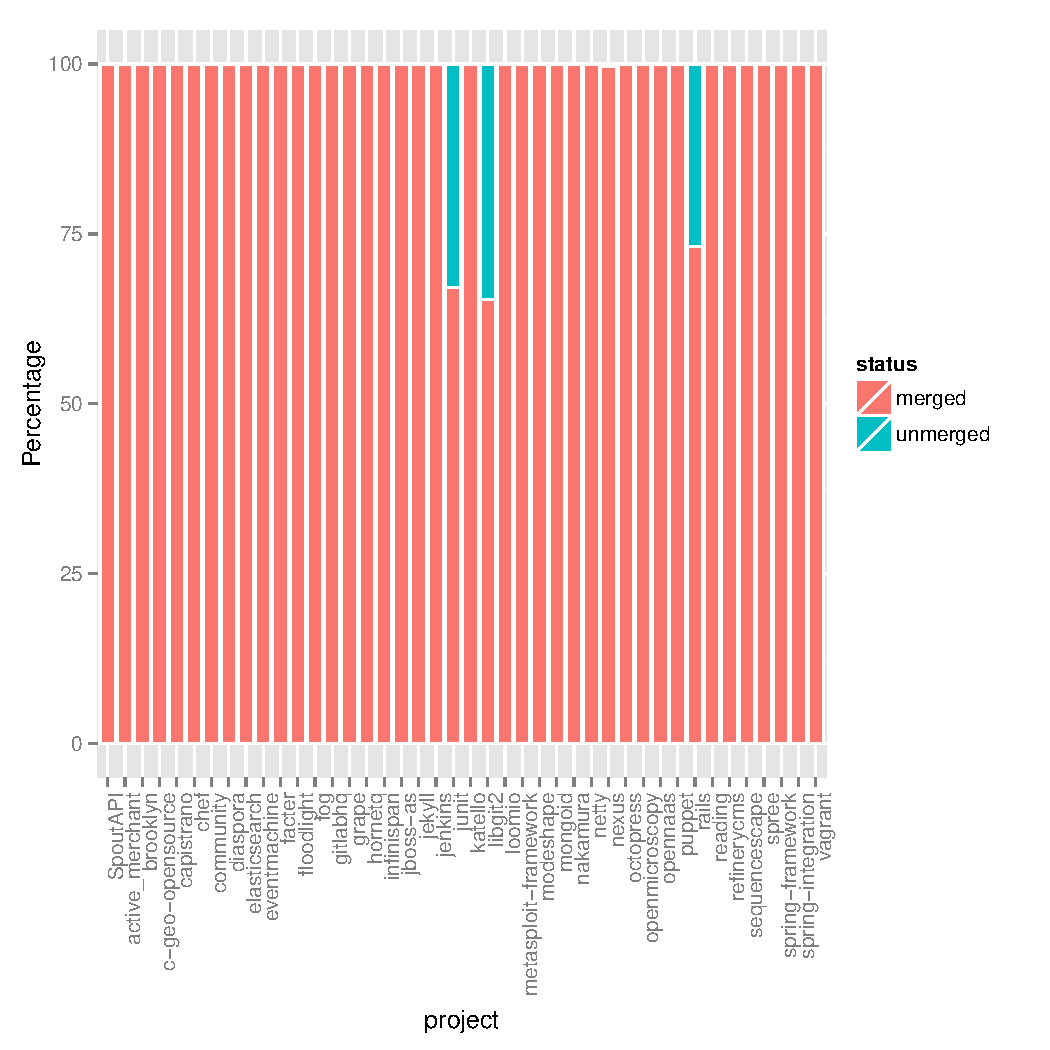
\includegraphics[scale=0.4]{perc-merged.pdf} 
  \label{fig:perc-merged}
}
\subfigure[Frequency distribution of lifetime for merged pull requests]{
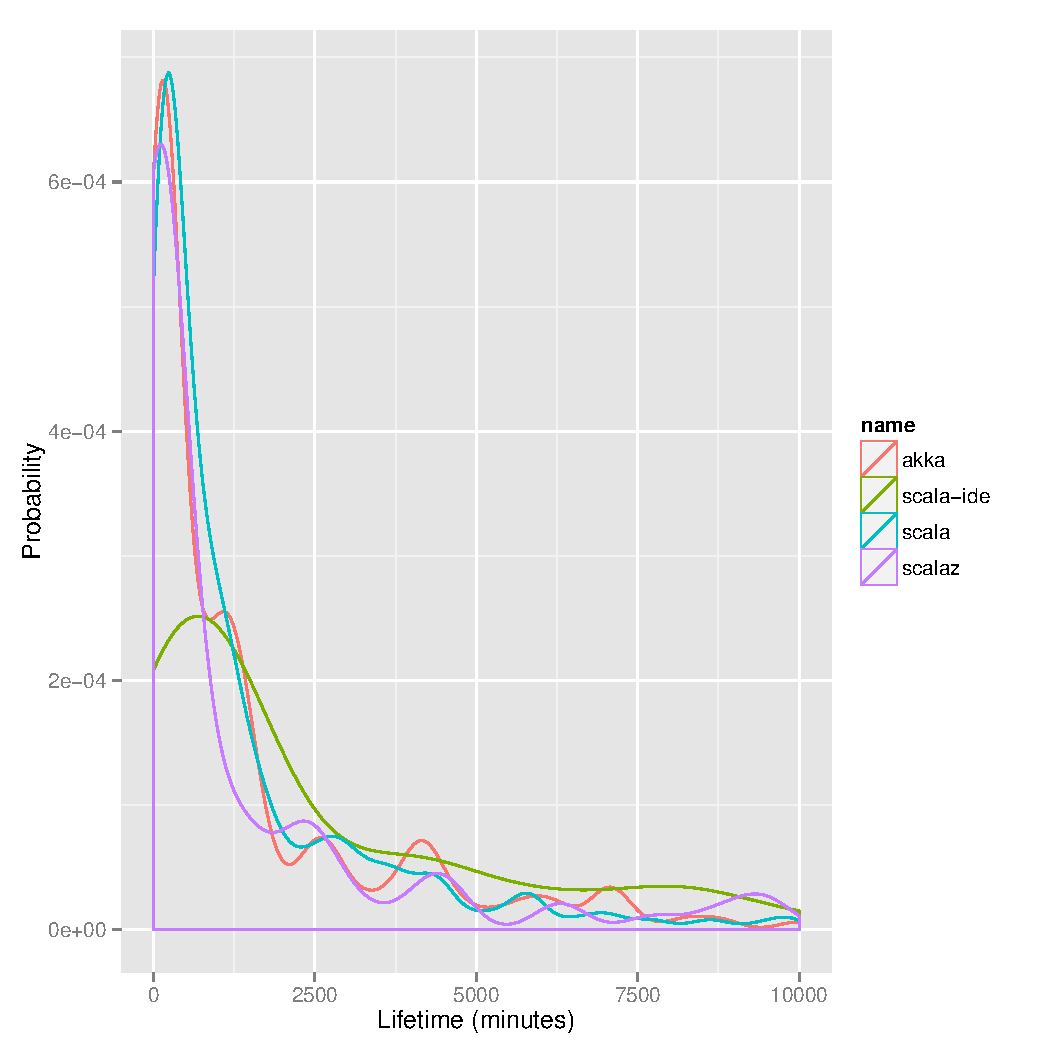
\includegraphics[scale=0.3]{lifetime-freq.pdf}
\label{fig:lifetime-freq}
}
\subfigure[Lifetime statistics for merged pull requests]{
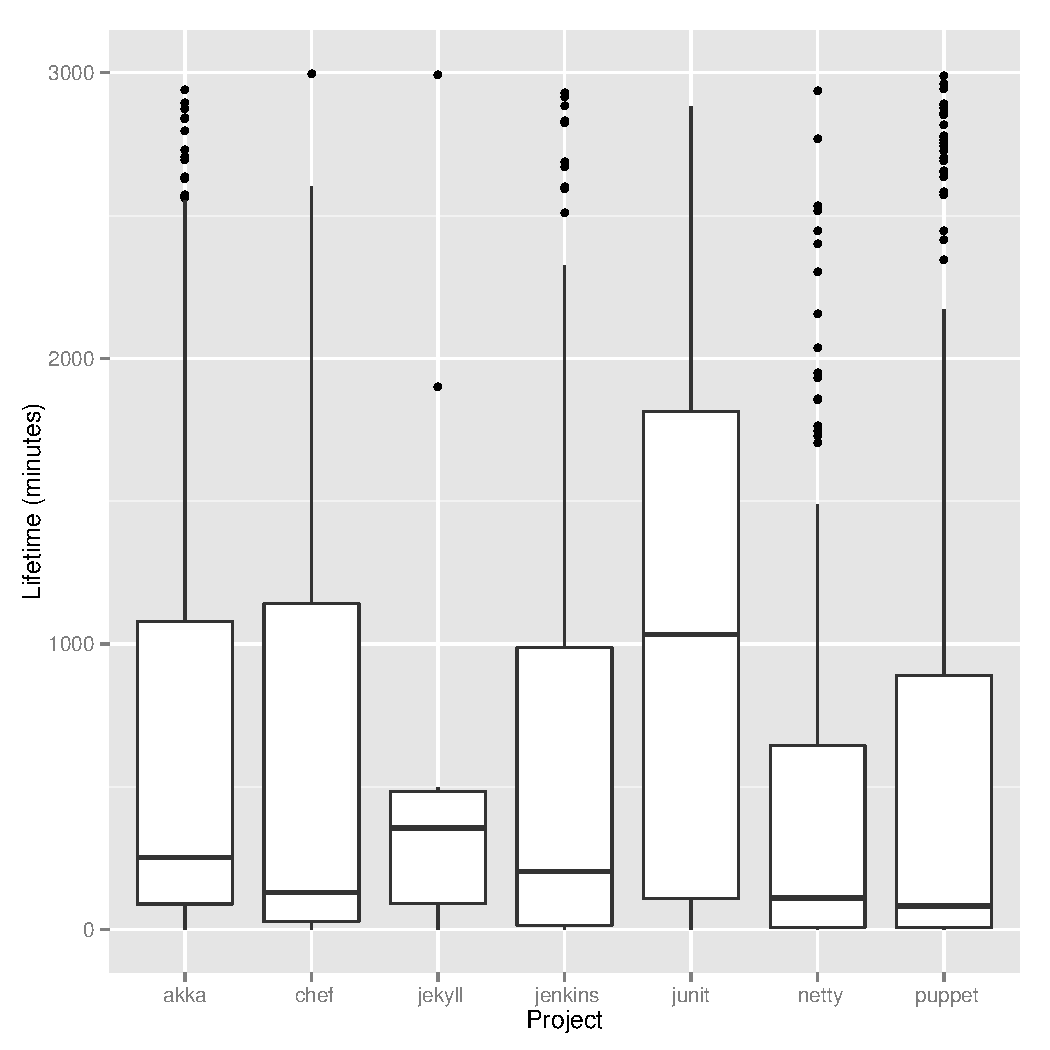
\includegraphics[scale=0.3]{lifetime-boxplot.pdf}
\label{fig:lifetime-boxplot}
}
\caption{Plots of pull request life time.}
\end{figure*}


An important observation is that there are several pull requests whose
lifetime is only limited to a ver

\subsection{Sizes of pull requests}

\subsection{Discussion and Code review}

Once a pull request has been submitted, it is open for discussion.

\subsection{Team size}

\subsection{Testing}

\section{Acceptance and rejection}

\begin{table*}
  \centering
  \begin{tabular}{rp{25em}}
    \hline
    \bf{Feature} & \bf{Description and Justification}\\
    \hline
    \multicolumn{2}{l}{\bf{Pull Request Impact}}\\
    
    \texttt{num\_commits} & Number of commits in the pull request. A bigger
    pull request will be slower to examine and therefore to merge.\\
    
    \texttt{churn} & Number of lines changed (added + deleted) by the pull request. The more lines changed, the longer a pull request will take to be
    reviewed.\\

    \texttt{files\_changed} & Number of files touched by the pull request. An
    indication of the impact of the pull request.\\
    
    \texttt{num\_commit\_comments} & Number of code review comments. More pull
    code review comments may indicate a rigorous process, therefore slowing down
    acceptance.\\
    
    \texttt{num\_issue\_comments} & Pull request discussion comments.\\

    \multicolumn{2}{l}{\bf{Project Characteristics}}\\
    
    \texttt{sloc} & Executable lines of code at pull request merge time. The
    bigger the project, the more difficult would be to assess the impact of
    a pull request\\

    \texttt{team\_size} & Number of active core team members during the last
    month prior the pull request merge. A big team will be faster to process a
    pull request as each team member will have less work load to handle and
    will be more specialized.\\

    \texttt{total\_commits\_last\_month} & Number of commits in the . Overall project activity indicator.\\
    
    \texttt{main\_team\_commits\_last\_month} & Activity of the main team
    members. An active main team will triage pull requests faster.\\

    \texttt{commits\_on\_files\_touched} & Activity on the files that are
    touched by the pull request. If the pull request touches files in a hotspot,
    it will be merged faster.\\
    
    \multicolumn{2}{l}{\bf{Effect of Testing}}\\

    \texttt{test\_churn} & Number of test lines in pull request. \\

    \texttt{asserts\_per\_1000\_lines} & A proxy for test coverage. The
    more well tested a project is, the easier and faster it will be to accept 
    a pull request.\\
    
    \multicolumn{2}{l}{\bf{Developer}}\\
    
    \texttt{requester} & The person that initiated the pull request.\\

    \texttt{num\_pullreqs} & Number of pull requests submitted by a specific
    developer, prior to the examined pull request. The more pull requests, the
    better the developer is known to the project.\\

    \texttt{is\_main\_team\_member} & Whether the developer belongs to the
    main repository team. Pull requests from main team members should be
    faster to accept and merge.\\
    \hline
  \end{tabular}
  \caption{Selected features}
  \label{tab:features}
\end{table*}

\section{Discussions and Conclusion}

\subsection{Threats to validity}

\section{Related Work}

\cite{Bird09}
\cite{Cornf10}
\cite{Dabbi12}
\cite{Bird12}
\cite{Barr12}
\cite{Buffe99}
\cite{Mens02}
\cite{Shiha12}

Global software development
\section{Conclusions}

\section*{Acknowledgements}
This work is partially supported by Marie Curie {\sc ief} 298930 -- {\sc sefunc}.

\bibliographystyle{ieeetr}
\bibliography{pullreqs}

\end{document}
